% -----------------------------------------------------------------
% Document class: Article
\documentclass[ a4paper, twoside, 11pt]{article}
\usepackage{../../macros-general}
\usepackage{../../macros-article}
% Number of the handout, quiz, exam, etc.
\newcommand{\numero}{03}
\setcounter{numero}{\numero}

% -----------------------------------------------------------------
\begin{document}
\allowdisplaybreaks

\begin{center}
\Large Sistemas de Control (EYAG-1005): Evaluaci\'on \numero \\[1ex]
\small \textbf{Semestre:} 2017-2018 T\'ermino I \qquad
\textbf{Instructor:} Jonathan Le\'on, Luis Reyes
\end{center}
\halfskip

\fbox{

\begin{minipage}[b][\height][t]{\textwidth}
\vspace{0.2 cm}

\begin{center}
\textbf{COMPROMISO DE HONOR}
\end{center}
\vspace{0.4 cm}

\scriptsize
{
Yo, \rule{60mm}{.1pt} al firmar este compromiso, reconozco que la presente lecci\'on est\'a dise\~nada para ser resuelta de manera individual, que puedo usar un l\'apiz o pluma y una calculadora cient\'ifica, \linebreak que solo puedo comunicarme con la persona responsable de la recepci\'on de la lecci\'on, y que cualquier instrumento de comunicaci\'on que hubiere tra\'ido debo apagarlo. Tambi\'en estoy conciente que no debo consultar libros, notas, \linebreak ni materiales did\'acticos adicionales a los que el instructor entregue durante la lecci\'on o autorice a utilizar. Finalmente, me comprometo a desarrollar y presentar mis respuestas de manera clara y ordenada. \\

Firmo al pie del presente compromiso como constancia de haberlo le\'ido y aceptado. 
\vspace{0.4 cm}

Firma: \rule{60mm}{.1pt} \qquad N\'umero de matr\'icula: \rule{40mm}{.1pt} \hspace{0.5cm} \\[-0.8ex]
}

\end{minipage}

}

\vspace{\baselineskip}



% =============================================
\begin{problem}
\textbf{[10 Puntos]} Encuentre la funci\'on de transferencia del siguiente sistema en t\'erminos de las funciones de transferencia $G_1(s), \, G_2(s) \, \dots, \, G_6(s)$, \ie la funci\'on: 
\[
G(s) \; \define \; \frac{\Theta_{22}(s)}{\Theta_{11}(s)}
\]
\begin{figure}[htb]
\centering
\includegraphics[ width = 0.88\textwidth]{fig_P5-8.jpg}
\end{figure}

\end{problem}
\vspace{\baselineskip}

% =============================================
\begin{problem}
\textbf{[10 Puntos]} Construya un modelo de espacio de estados para el siguiente sistema mec\'anico rotacional donde la entrada es el torque $T(t)$ y la salida es la posici\'on angular del cuerpo del lado izquierdo (el que tiene inercia de 3 kg-m\tsup{2}). Por conveniencia, por favor denote el \'angulo del cuerpo del lado izquierdo como $\theta_0(t)$, el del cuerpo del lado derecho superior como $\theta_1(t)$, y el del cuerpo del lado derecho inferior como $\theta_2(t)$. 

\begin{figure}[htb]
\centering
\includegraphics[ width = 0.62\textwidth]{fig_P2-20.jpg}
\end{figure}

\end{problem}
\vspace{\baselineskip}

% =============================================
\begin{problem}
Considere un sistema cuya respuesta de la frecuencia es como se muestra en la figura de abajo. 

\begin{figure}[H]
\centering
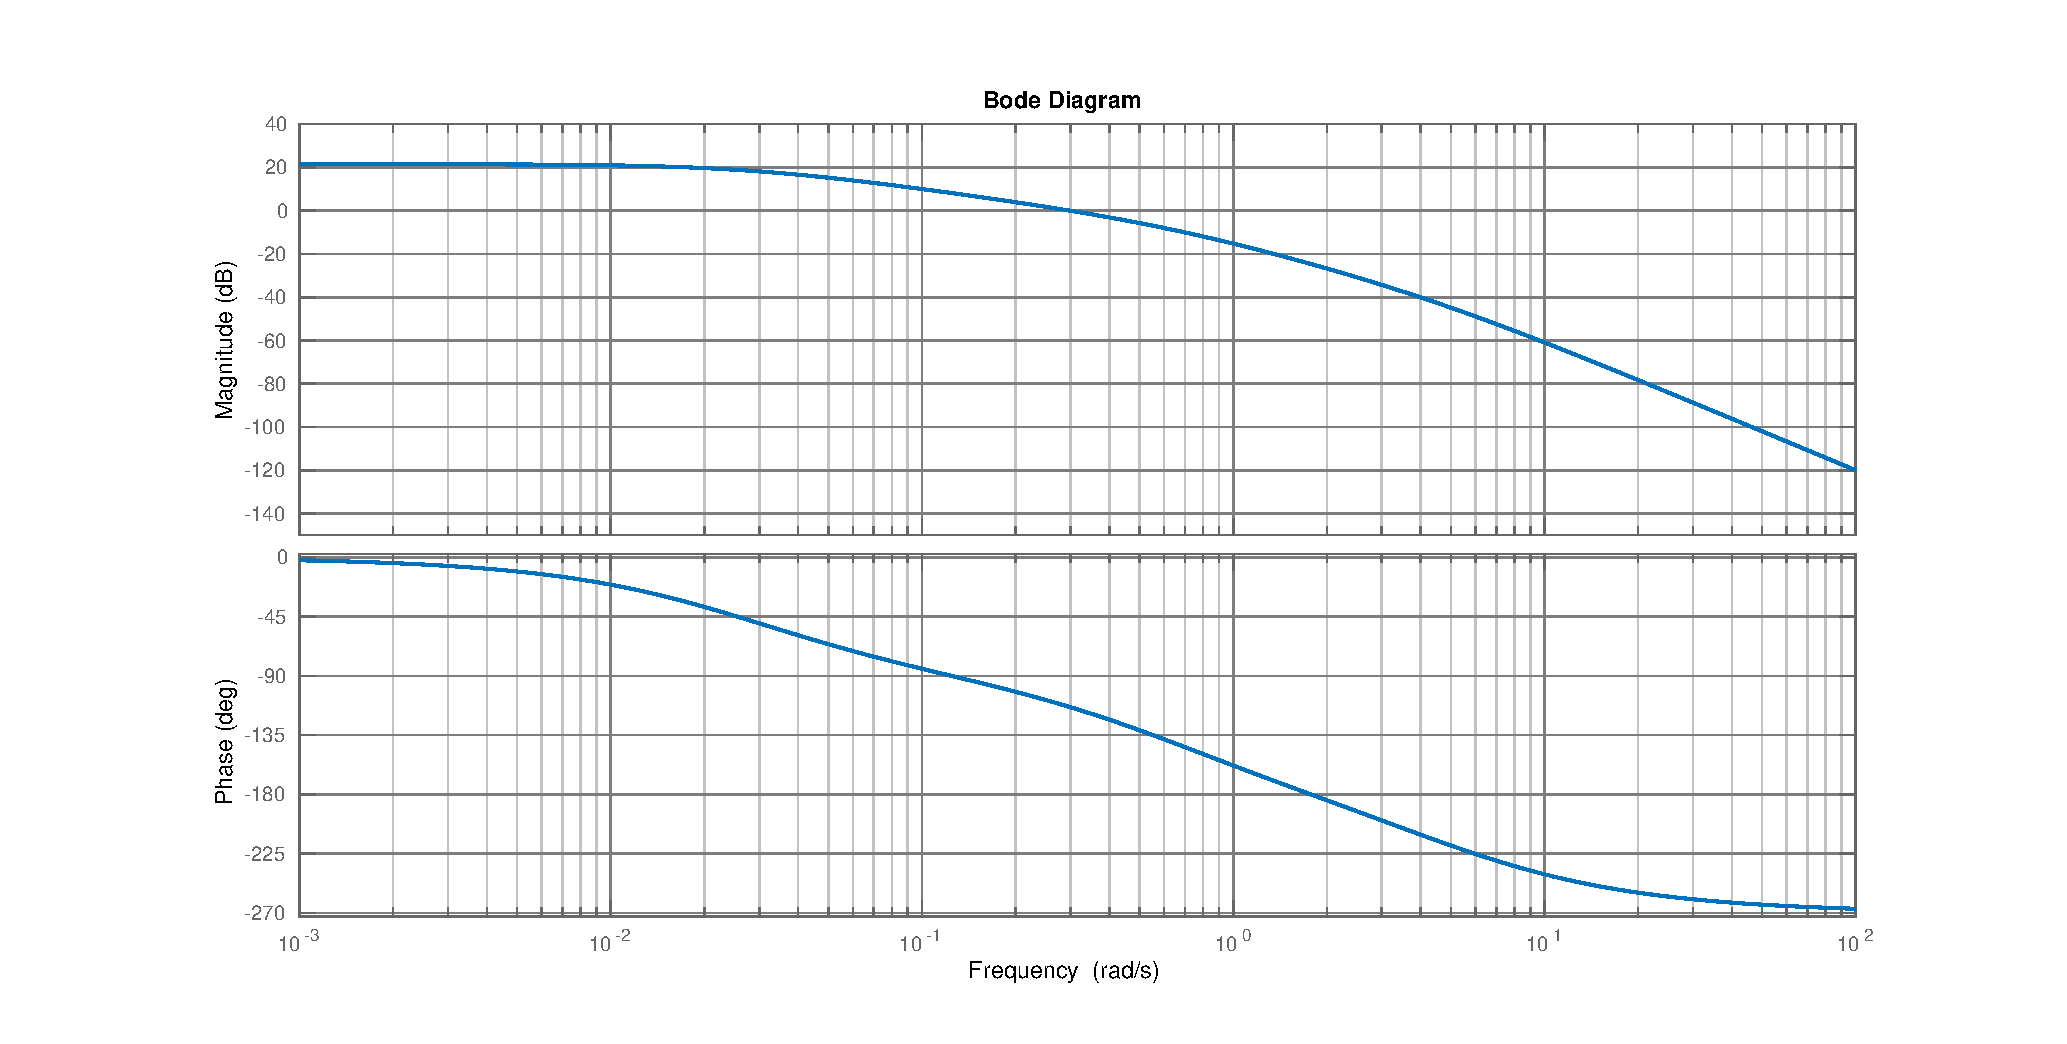
\includegraphics[width=\columnwidth]{problema-bode.eps}
\end{figure}

Con esto en mente, complete las siguientes actividades: 
\begin{enumerate}[label=\alph*.]
\item \textbf{[4 Puntos]} Calcule los m\'argenes de ganancia y fase del sistema.
\item Suponiendo que el sistema es puesto en un lazo de retro-alimentaci\'on unitaria, compute las siguientes m\'etricas de desempe\~no del sistema en circuito cerrado: 
\begin{itemize}
\item \textbf{[3 Puntos]} Error en estado estable para una entrada escal\'on.
\item \textbf{[3 Puntos]} Porcentage de sobrepaso. Puede utilizar la curva mostrada en la figura de abajo para realizar sus c\'alculos. 
\begin{figure}[htb]
\centering
\includegraphics[width=0.72\textwidth]{Fig_phase-damping.jpg}
\end{figure}

\end{itemize}
\end{enumerate}

\end{problem}
\vspace{\baselineskip}

\end{document}
